% ======================================================
%  2 — DATASET
% ======================================================

\section[The Dataset]{The Dataset: 125,600 Italian Clue--Answer Pairs}
% --- 2.1 Overview ---
\begin{frame}{Building a Large-Scale Linguistic Resource}
  \begin{columns}[c]
    \column{0.42\textwidth}
      \begin{center}
        {\fontsize{44}{52}\selectfont\color{unisired}\textbf{125,600}}\\[0.3em]
        {\large unique clue--answer pairs}\\[1.5em]
        {\normalsize\color{graytext} Sources:}\\[0.3em]
        {\small Dizy.com, Cruciverba.it,\\
        La Settimana Enigmistica,\\
        La Repubblica}
      \end{center}
    \column{0.58\textwidth}
      \centering
      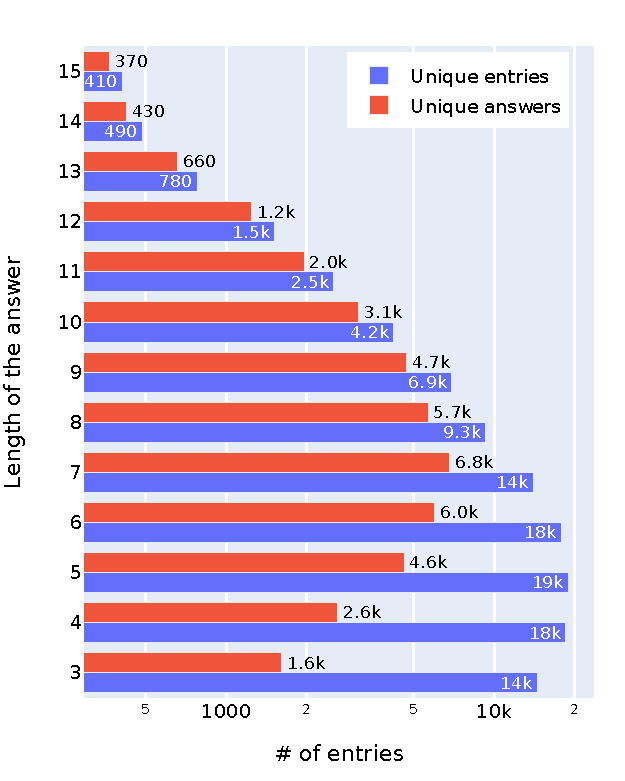
\includegraphics[width=\textwidth, height=0.72\textheight, keepaspectratio]{figures/italian_db.pdf}
  \end{columns}
  \vfill
  {\scriptsize\color{graytext} Publicly available:
  \url{https://github.com/tommyiaq/cruciverba} --- CC BY-NC 4.0}
\end{frame}

% --- 2.1b English dataset ---
\begin{frame}{Also: An English Dataset}
  \begin{columns}[c]
    \column{0.42\textwidth}
      \begin{center}
        {\fontsize{44}{52}\selectfont\color{unisired}\textbf{7.3M}}\\[0.3em]
        {\large clue--answer entries}\\[1.5em]
        {\normalsize\color{graytext} $\sim$300,000 unique answers}\\[0.4em]
        {\small 1913--2021 · web scraping\\
        + manual extraction}
      \end{center}
    \column{0.58\textwidth}
      \centering
      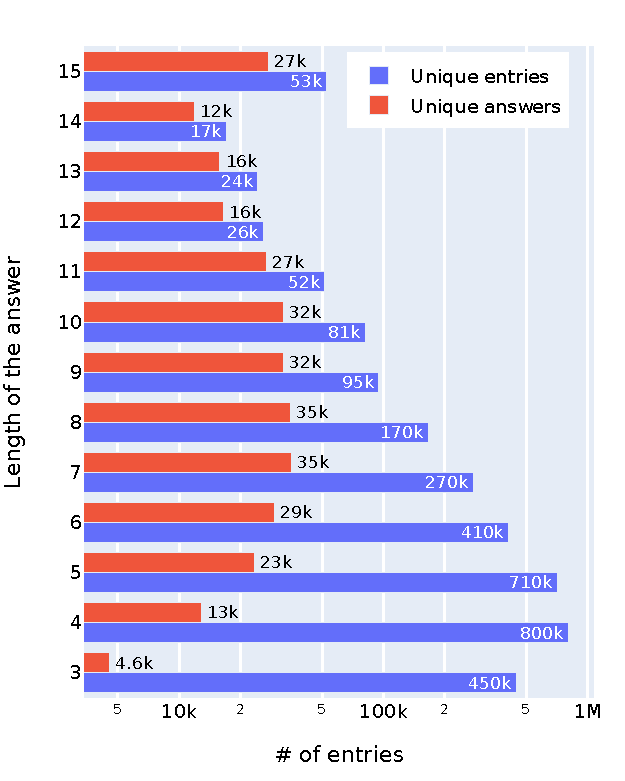
\includegraphics[width=\textwidth, height=0.72\textheight, keepaspectratio]{figures/english_db.pdf}
  \end{columns}
  \vfill
\end{frame}

% --- 2.2 Linguistic typology ---
\begin{frame}{Five Ways to Write a Clue}
  \vspace{0.2em}
  \begin{tikzpicture}
    % Each row: bar + % label + Italian example + English gloss
    % --- Row 1: Nominal 46% ---
    \fill[unisired]      (0, 4.0) rectangle (4.00, 4.32);
    \node[left,  font=\small\bfseries, text=darktext,  anchor=east] at (0, 4.16) {Nominal};
    \node[right, font=\scriptsize,     text=white,     anchor=west] at (0.1, 4.16) {46\%};
    \node[right, font=\small,          text=graytext,  anchor=west] at (4.2, 4.16)
      {\textit{Infuso paglierino} $\rightarrow$ \textbf{tè}};
    \node[right, font=\scriptsize\itshape, text=graytext, anchor=west] at (4.2, 3.72)
      {(straw-coloured infusion $\rightarrow$ tea)};
    % --- Row 2: Verbal 21% ---
    \fill[unisired!75]   (0, 3.0) rectangle (1.83, 3.32);
    \node[left,  font=\small\bfseries, text=darktext,  anchor=east] at (0, 3.16) {Verbal};
    \node[right, font=\scriptsize,     text=white,     anchor=west] at (0.1, 3.16) {21\%};
    \node[right, font=\small,          text=graytext,  anchor=west] at (4.2, 3.16)
      {\textit{Risiede in uno spazio geografico} $\rightarrow$ \textbf{abitante}};
    \node[right, font=\scriptsize\itshape, text=graytext, anchor=west] at (4.2, 2.78)
      {(lives in a specific geographic area $\rightarrow$ inhabitant)};
    % --- Row 3: Metalinguistic 12% ---
    \fill[unisired!55]   (0, 2.0) rectangle (1.04, 2.32);
    \node[left,  font=\small\bfseries, text=darktext,  anchor=east] at (0, 2.16) {Metalinguistic};
    \node[right, font=\scriptsize,     text=darktext,  anchor=west] at (0.1, 2.16) {12\%};
    \node[right, font=\small,          text=graytext,  anchor=west] at (4.2, 2.16)
      {\textit{Il centro di Matera} $\rightarrow$ \textbf{TE}};
    \node[right, font=\scriptsize\itshape, text=graytext, anchor=west] at (4.2, 1.82)
      {(letter-game: center of ``Ma\underline{TE}ra'')};
    % --- Row 4: Adjectival 9% ---
    \fill[unisired!40]   (0, 1.0) rectangle (0.78, 1.32);
    \node[left,  font=\small\bfseries, text=darktext,  anchor=east] at (0, 1.16) {Adjectival};
    \node[right, font=\scriptsize,     text=darktext,  anchor=west] at (0.1, 1.16) {9\%};
    \node[right, font=\small,          text=graytext,  anchor=west] at (4.2, 1.16)
      {\textit{Probo, retto} $\rightarrow$ \textbf{onesto}};
    \node[right, font=\scriptsize\itshape, text=graytext, anchor=west] at (4.2, 0.82)
      {(upright, straight $\rightarrow$ honest)};
    % --- Row 5: Copular 5% ---
    \fill[unisired!25]   (0, 0.0) rectangle (0.44, 0.32);
    \node[left,  font=\small\bfseries, text=darktext,  anchor=east] at (0, 0.16) {Copular};
    \node[right, font=\scriptsize,     text=darktext,  anchor=west] at (0.1, 0.16) {5\%};
    \node[right, font=\small,          text=graytext,  anchor=west] at (4.2, 0.16)
      {\textit{Fu Cancelliere dal 1949 al 1963} $\rightarrow$ \textbf{Adenauer}};
    \node[right, font=\scriptsize\itshape, text=graytext, anchor=west] at (4.2, -0.22)
      {(was Chancellor from 1949 to 1963)};
  \end{tikzpicture}
  \vfill
  {\small\color{graytext}\textit{Nominal phrases alone cover nearly half the dataset --- Italian crosswords favour concise lexical definitions over full sentences.}}
\end{frame}